% !TEX program=pdflatex
% !BIB program=biber

\documentclass[USenglish,oneside,twocolumn]{article}
%\selectlanguage{en}

\usepackage[T1]{fontenc}
\usepackage[utf8]{inputenc}%(only for the pdftex engine)
%\RequirePackage[no-math]{fontspec}%(only for the luatex or the xetex engine)
\usepackage[big]{dgruyter_NEW}
% \fancyhf{} % Remove fancy page headers 
% \fancyhead[C]{Anonymous submission \#9999 to ACM CCS 2019} % TODO: replace 9999 with your paper number
% \fancyfoot[C]{\thepage}

% \setcopyright{none} % No copyright notice required for submissions
% \acmConference[Anonymous Submission to ACM CCS 2020]{ACM Conference on Computer and Communications Security}{Due 20 January 2020}{Orlando, TBD}
% \acmYear{2019}

% \settopmatter{printacmref=false, printccs=true, printfolios=true} % We want page numbers on submissions
 
% \usepackage{cite}
% \bibliographystyle{apa}
\usepackage{amsmath} 
\usepackage{amsthm} 
\usepackage{amsfonts}
\usepackage{graphicx}
\usepackage{booktabs}
\usepackage{caption}
\usepackage{subcaption}
\usepackage{lmodern}
\usepackage{framed}
\usepackage{mathtools}
\usepackage{float} 
\usepackage{algorithmicx}   
\newtheorem{theorem}{Theorem}[section] 
\newtheorem{definition}{Definition}[section]
\newtheorem{corollary}{Corollary}[theorem]
\newtheorem{lemma}[theorem]{Lemma}
%\usepackage{cochineal}
%\usepackage[activate={true,nocompatibility},final,tracking=true,kerning=true,factor=1100,stretch=0,shrink=10]{microtype}
\usepackage{algpseudocode}
\linespread{0.96}
%\usepackage{xcolor} \pagecolor[rgb]{0.2,0.2,0.2} \color[rgb]{1,1,1}

% \makeatletter
% \def\@IEEEsectpunct{.\ \,}
% \def\paragraph{\@startsection{paragraph}{4}{\z@}{1.5ex plus   
% 0.5ex minus .2ex}{-0em}{\normalsize\bf}}
% \makeatother

\newcommand{\mathcoin}[2]{\langle #1 \rightarrow #2 \rangle}
\newcommand{\mathcoinu}[2]{\ell_{#1 \rightarrow #2}}
\newcommand{\Astrape}[0]{\textsc{Astrape}}

\algtext*{EndFunction}% Remove "end while" text
\algtext*{EndFor}% Remove "end if" text
\algtext*{EndIf}
 
%\renewcommand{\baselinestretch}{1.06}
\begin{document}

\title{Astrape: Anonymous Payment Channels with Boring Cryptography}
%\author{\IEEEauthorblockN{Yuhao Dong\IEEEauthorrefmark{1} and
%Raouf Boutaba\IEEEauthorrefmark{2}}
%\IEEEauthorblockA{Cheriton School of Computer Science,
%University of Waterloo\\
%Waterloo, Canada\\
%Email: \IEEEauthorrefmark{1}yd2dong@uwaterloo.ca,
%\IEEEauthorrefmark{2}rboutaba@uwaterloo.ca}}
\maketitle

\begin{abstract}
    Increasing use of blockchain-based cryptocurrencies like Bitcoin and Ethereum have run into inherent scalability limitations of blockchains. Payment channel networks, or PCNs, promise to greatly increase scalability by conducting the vast majority of transactions outside the blockchain while leveraging it as a final settlement protocol. Unfortunately, currently deployed PCNs have significant flaws in security and privacy. In particular, even though transactions are conducted off-chain, anonymity guarantees are very weak.

    In this work, we present Astrape, a novel PCN construction that achieves strong security and anonymity guarantees with simple, black-box cryptography. Existing anonymous PCN constructions all integrate with specific, often custom-designed, cryptographic constructions, but Astrape can use any generic public-key signature scheme and any random-oracle hash function. This allows Astrape to achieve provable security without relying on any specific computational hardness assumption. Astrape's simple cryptography also lends itself to unusually straightforward security proofs compared to existing systems.

    Furthermore, we evaluate Astrape's performance, including that of a concrete implementation on the Bitcoin Cash blockchain. We show that on the average case, Astrape operations require less than 20 milliseconds of computation and 1 KB of communication on commodity hardware. Astrape explores a novel avenue to secure and anonymous PCNs that achieves similar or better performance compared to all existing solutions.
\end{abstract}

\section{Introduction}

\subsection{Payment channel networks}

Blockchain-based cryptocurrencies, like Bitcoin, Litecoin, and DASH, are gaining in popularity and becoming a significant alternative to traditional government-issued money. For instance, almost 300,000 Bitcoin transactions alone \cite{bccom} are processed every day. Unfortunately, such high demand inevitably causes blockchain cryptocurrencies to run into well-known scalability barriers \cite{croman2016scaling}. In Bitcoin's case, less than 10 transactions per second in total can be processed \cite{mccorry2016towards}, far less than the throughput required for a global payment system.

\emph{Payment channels} \cite{decker2015fast} have become the most common way in practice of scaling cryptocurrency transactions. In a nutshell, Alice and Bob open a payment channel by submitting a single transaction to the blockchain, that locks up a sum of cryptocurrency from both of the parties. They can then perform payments to each other without using the blockchain, by simply mutually agreeing on which portion of the locked money belongs to Alice and which to Bob. Additional blockchain transactions are required only when the channel is closed, unlocking the latest balances of Alice and Bob on the blockchain. Payment channels solve blockchains' scalability problem by allowing the vast majority of transactions to be conducted outside the blockchain, yet retaining the blockchain for final settlement: as long as the blockchain is secure, nobody can steal funds.

More importantly, payment channels can be organized into \emph{payment-channel networks} (PCNs) \cite{mccorry2016towards}, where users without any open channels between them can pay each other through intermediaries that they do have open channels to. This allows horizontally scalable payment networks based on trustless off-chain settlement, vastly improving the usability of decentralized cryptocurrencies. Despite some disadvantages, most importantly the capital inefficiency of locking up funds in channels, PCNs are widely considered a promising avenue for scalable cryptocurrency payments.

\subsection{Anonymity in PCNs}

Unfortunately, ``first-generation'' PCNs based on the HTLC (hash time-locked contract), such as Lightning Network \cite{decker2015fast} and Raiden \cite{raiden}, have a significant problem --- poor anonymity \cite{malavolta2017concurrency}. The very contracts that ensure blockchain-tied security also make payments in the worst case as transparently linkable as blockchain payments \cite{malavolta2017concurrency}, since HTLC uses a unique hash preimage to identify each overall transaction. This threatens the improved privacy compared to on-chain transactions that is often cited as a benefit of PCNs. Furthermore, naive implementations fall victim to subtle fee-stealing attacks, like the ``wormhole attack'' \cite{malavolta2019anonymous}, that threaten the viability of large PCNs.

A sizable body of existing work on fixing PCN security and privacy exists, mostly divided into two groups. On one hand, specialized constructions can achieve strong anonymity in specific settings, such as Bolt \cite{green2017bolt} for hub-based PCNs on the ZCash blockchain. These specialized solutions typically provide for indistinguishability of two concurrent transactions even when all intermediaries are malicious. On the other hand, general solutions for all PCN topologies, like AMHL \cite{malavolta2019anonymous} and Fulgor \cite{malavolta2017concurrency}, achieve a somewhat weaker, topology-dependent notion of anonymity: \emph{relationship anonymity} \cite{backes2013anoa}. This property, common to onion-routing and other anonymous communication protocols, means that two concurrent transactions cannot be distnuished as long as they share at least one honest intermediary.

Unfortunately, all existing systems share one weakness. No existing anonymous PCN construction limits itself to the bare-bones cryptographic primitives used in HTLC --- black-box access to a generic signature scheme and hash function. Instead, almost all existing anonymous payment channel networks are tightly coupled to the mathematics of specific cryptographic constructions. Tumblebit \cite{heilman2017tumblebit}, for instance, uses a custom cryptosystem based on the RSA assumption. Systems that do use black-box primitives nevertheless require fairly exotic and difficult-to-implement primitives, such as the non-interactive zero-knowledge proofs used in Fulgor \cite{malavolta2017concurrency}.

In the case of the first group of anonymous PCNs, this is understandable, as total unlinkability is a difficult goal to achieve, and likely impossible without some sort of zero-knowledge proof in settings like a hub-based PCN with one, untrusted hub. PCN constructions based on relationship anonymity, however, have no such excuse. First of all, relationship anonymity appears to be a relatively weak property for a cryptosystem to achieve. Standard and well-understood relationship-anonymous constructs, like onion routing and mix networks, exist for communication with no more than standard black-box primitives used in secure communication (symmetric and asymmetric encryption). \emph{Prima facie}, use of exotic cryptographic constructs to merely achieve relationship anonymity seems to be overkill.

Use of custom cryptography when not needed is not a merely academic problem. Black-box cryptography allows easy replacement of cryptographic primitives without wholesale protocol redesign, making it much easier to deal with possible breakthroughs in cryptanalysis or computation (e.g. practical quantum computers). For example, we can easily replace ECDSA in Bitcoin with any unforgeable signature scheme or AES in TLS with any secure block cipher, without compromising their security or requiring their wholesale redesign. This is simply not possible with existing anonymous PCNs. Tumblebit \cite{heilman2017tumblebit}, for instance, uses a custom cryptosystem based on the RSA assumption, and if RSA were to be broken, Tumblebit's entire design collapses. Furthermore, a black-box design allows us to seamlessly replace cryptographic primitives (like RSA) with more efficient but mathematically different primitives  with the same properties (like elliptic curves). Finally, black-box cryptography makes provable security easier, as we can rely on high-level properties of the black-box primitives (such as unforgeability of a signature scheme) rather than only using low-level computational hardness assumptions.

Thus, we believe that any relationship-anonymous PCN construction should strive towards using ``boring'' cryptography --- black-box, pervasively used cryptographic primitives.

\subsection{Our contributions}

In this paper, we present Astrape, the first PCN protocol that uses entirely ``boring'' cryptography yet achieves strong relationship anonymity. Despite achieving comparable security, privacy, and performance to other anonymous PCN constructions, Astrape does not introduce any cryptographic constructs other than those used in HTLC.

\begin{itemize}
    \item We discuss existing payment channel networks, focusing on their security and privacy properties. In particular, we show that PCNs based on the hash time-lock contract (HTLC), such as Lightning Network, have significant privacy and security problems. We discuss existing work on improving PCNs and their extensive reliance on either specialized environments or novel cryptographic constructions.
    \item We introduce a formal model of PCN constructions, ``generalized multi-hop locks'' (GMHL), based on existing work defining ``anonymous multi-hop locks''~\cite{malavolta2019anonymous}. that generalizes all sorts of PCN constructs. We model the security and privacy properties we desire from a PCN construction within this model.
    \item Within the GMHL framework, we introduce Astrape, a new PCN construction that solves the security and privacy issues of HTLC-based constructs with only black-box cryptographic primitives. Strong privacy without new cryptographic primitives solves an important open problem in the field. Astrape builds upon existing work \cite{malavolta2017concurrency} on private PCNs but uses a new technique that avoids the need for zero-knowledge proofs. We prove that Astrape fulfills all of our security and privacy goals, even with very powerful adversaries.
    \item We implement Astrape and show that on average, Astrape requires less computation or communication than state-of-the-art private PCN constructions. We show that Astrape can easily be ported to different blockchains, due to its use of standard cryptographic primitives and the generality of the GMHL model.
\end{itemize}


\section{Background and related work} \label{sec:bg}

\subsection{Payment channels}

The fundamental building block of payment channel networks is the bilateral payment channel \cite{mccorry2016towards}. A payment channel is a construct where two parties Alice and Bob deposit money into a blockchain-enforced ``vault'' that can be only opened with signatures from both Alice and Bob. Alice and Bob can then send each other money by privately agreeing on the distribution of funds between them by signing dated statements that split the money between them, without using the blockchain at all. When the funds locked in the vault are insufficient, or one of the parties need to access the funds, one of the parties can simply open the vault using any statement signed by both parties that was produced in the course of using the payment channel, subject to a short period of time where the other party may override the statement with a later-dated statement. This mechanism ensures security of funds even if one of the parties is malicious.

\subsection{Multi-hop networks with HTLC}

An extremely useful property of payment channels is that they can be used to construct \emph{payment channel networks} (PCNs) \cite{mccorry2016towards,decker2018eltoo,croman2016scaling}. A PCN is simply a directed graph of payment channels between users, allowing users without payment channels directly between each other to pay each other by routing the money over intermediaries. For example, the Lightning Network, one of the most prominent PCNs, has over 30,000 channels connecting more than 4,000 nodes \cite{github2019lnd}. Any of these 4,000 nodes can pay any other.

A crucial building block of secure PCNs is the \emph{secure multi-hop transaction} (SMHT) --- some way of Alice paying Bob to pay Carol without any trust in Bob. Most PCNs implement an SMHT using a smart contract known as the \emph{Hash Time-Lock Contract} (HTLC). An HTLC is parameterized over a \emph{sender} Alice, the \emph{recipient} Bob, a deadline $t$, and a \emph{puzzle} $s$. It locks up a certain amount of money, unlocking it according to the following rules:
\begin{itemize}
    \item The money goes to Bob if he produces $\pi$ where $H(\pi) = s$ before time $t$, where $H$ is a secure hash function.
    \item Otherwise, the money goes to Alice.
\end{itemize}

HTLCs are used to implement an SMHT in the following way. Consider a sender $U_0$ wishing to send money to a recipient $U_n$ through untrusted intermediaries $U_0,\dots,U_n$. At first, $U_0$ will generate a random $\pi$ and $s=H(\pi)$, while sending the pair $(\pi,s)$ to $U_n$ over a secure channel (for instance, encrypted under $U_n$'s public key and transmitted over the Tor \cite{dingledine2004tor} network). $U_0$ can then lock money in a HTLC parameterized over $U_0,U_1,s,t_1$, notifying $U_1$. $U_1$ would send an HTLC over $U_1,U_2,s,t_2$, notifying $U_2$, and so on. The deadline must become earlier at each step --- $t_1>t_2>\dots>t_n$ --- this ensures that in case of an uncooperative or malicious intermediary, funds always revert to the sender.

The payment eventually will be routed to $U_n$, who will receive an HTLC over $U_{n-1},U_n,s$. He will claim the money by providing $\pi$; this allows $U_{n-1}$ to claim money from $U_{n-2}$ using the same $\pi$, and so on, until all outstanding HTLC contracts are fulfilled. $U_0$ has successfully sent money to $U_n$, while the preimage resistance of $H$ prevents any intermediary from stealing the funds.

\subsection{Hub-based anonymous payment channels}

An important property we may want from PCNs is strong anonymity. Intuitively, taking transactions away from the prying eyes of the public blockchain should enable two parties to transact without risking third-party surveillance. Unfortunately, HTLC has an inherent privacy problem --- a common identifier $s=H(\pi)$ visible to all nodes in the payment path. Even when the communications between all PCN nodes are done over a robust anonymizing protocol, this property still severely hampers privacy \cite{green2017bolt,malavolta2017concurrency,malavolta2019anonymous}. Furthermore, when payment channels are closed and transactions end up settling on the blockchain, privacy degenerates to be similar to that of on-chain transactions.

\emph{Hub-based} approaches form the earliest and most common kind of anonymous PCN design. In a hub-based anonymous PCN, the shape of the network is limited to a star topology with users communicating with a centralized (though typically untrusted) hub. Many of these networks are highly specialized, such as Green and Miers' BOLT \cite{green2017bolt}, which relies on the Zcash blockchain's zero-knowledge cryptography, and Lind and Eyal's Teechain design \cite{lind2016teechan}, which uses trusted execution environments. Other hub-based approaches, such as Tumblebit \cite{heilman2017tumblebit} and the more recent A2L \cite{tairi2019a2l}, provide more general solutions that work on a wide variety of blockchains.

Hub-based PCN constructions tackle the inherently difficult problem of providing unlinkability between transactions despite the existence of only one, global, untrusted intermediary. It is therefore no surprise that highly specialized cryptography is needed to protect anonymity. Fortunately, actual payment channel networks often have intricate topologies with many participants and no huge hubs. General, topology-agnostic solutions, which may not need the kind of cryptography common in hub-based approaches, are thus more important to deploying private PCNs in practice.

\subsection{Relationship-anonymous payment channels}

Unlike hub-based approaches, where no intermediaries are trusted (since there is only one), general private PCN constructions target \emph{relationship anonymity}. This concept, which these constructions share with onion routers and other anonymous communication protocols, assumes the existence of at least one honest intermediary between the counterparties. Thus intermediaries are in fact crucial to relationship-anonymous PCNs' privacy properties, since they achieve privacy by bouncing the payment between multiple non-colluding parties.

The earliest solution to PCN privacy in this family was probably Fulgor and Rayo \cite{malavolta2017concurrency}, a closely related pair of constructions that can be ported to almost all HTLC-based PCNs. Fulgor/Rayo combines a ``multi-hop HTLC'' contract with out-of-band zero-knowledge proofs to remove the common identifier between different hops of the payment.

More recently, Malavolta et al. \cite{malavolta2019anonymous} introduced \emph{anonymous multi-hop locks} (AMHL), a rigorous theoretical framework for analyzing private PCN contracts. The AMHL paper provided a concrete instantiation using linear homomorphic encryption, which provides significant performance benefits compared to systems based on zero-knowledge like BOLT or Fulgor/Rayo, while conjecturing that linear homomorphic encryption is necessary for implementing anonymous PCNs. They also presented a clever way of encoding homomorphic encryption in terms of ECDSA, allowing AMHL to be used in traditional blockchains like Bitcoin.

Another important contribution by the authors of AMHL was the discovery of ``wormhole attacks'' on HTLC-based PCNs. These attacks exploit a fundamental flaw in the HTLC construction to allow malicious intermediaries to steal transaction fees from honest ones. It turns out that anonymity techniques to remove the common HTLC identifier also take care of fixing this class of attack, making research into anonymous non-HTLC payment channel contracts worthwhile not only for privacy but also security improvements.

\begin{figure*}
    \centering
    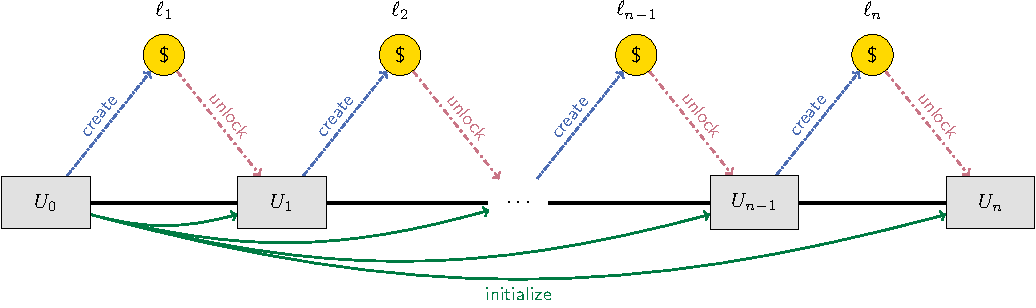
\includegraphics[width=0.8\textwidth]{graphics/coinpassing.pdf}
    \caption{An illustration of the GMHL model}
    \label{fig:coinpassing}
\end{figure*}

\subsection{Why a new solution?}

Ever since HTLCs were first proposed, anonymous PCNs solutions have progressed greatly. Systems like AMHL and A2L achieve rigorous anonymity guarantees without significantly sacrificing performance, while keeping compatibility with many existing blockchains. It is easy to conclude that anonymous payment channels are a mostly ``solved problem''.

Yet there remains a weakness common to all existing anonymous PCN constructions --- reliance on custom cryptographic primitives. For example, AMHL uses linear homomorphic encryption, Fulgor uses non-interactive zero-knowledge proofs, and Tumblebit uses a custom cryptosystem based on the RSA assumption. Although these constructs are typically based on commonly accepted cryptographic assumptions, this situation is still not ideal.

First, non-standard cryptography poses barriers to adoption. Portability is reduced --- AMHL's clever embedding of homomorphic encryption within ECDSA does not extend to other signature schemes, for example. More importantly, reliable and performant implementations of novel cryptographic functions are also difficult to obtain. Widely used, well-audited cryptographic libraries like libsodium \cite{libsodium} or OpenSSL \cite{openssl} generally neither implement functions such as RSA-based homomorphic encryption nor provide tools to securely implement them.

Furthermore, tight coupling between a PCN protocol and the mathematics of a particular cryptographic construction makes swapping out cryptographic primitives impossible. For example, Tumblebit's cryptography crucially depends on RSA's algebraic structure \cite{heilman2017tumblebit}. In case RSA is broken through practical quantum computers or advances in factorization, Tumblebit must be completely redesigned, but with use of black-box cryptography, we can simply upgrade to quantum-safe primitives.

Thus, we believe that finding a way of constructing efficient yet privacy-preserving PCNs by composing well-understood and easily replaced black-box cryptographic primitives is crucial to usable anonymous payment channels. In fact, AMHL's authors already posed finding the minimal set of cryptographic primitives as an ``interesting problem'' \cite{malavolta2019anonymous} that they conjecturally answered with linear homomorphic encryption.

Astrape is our solution to the problem of cryptographically simple anonymous PCNs that refutes this conjecture. We show that anonymous and atomic multi-hop transactions can be constructed with nothing but the two building blocks of HTLCs --- hashing and signatures. Unlike existing a work, no mathematical assumptions about the structure of the hash function or signature scheme are made, allowing Astrape to be easily ported to different concrete cryptographic primitives and its security properties to ``fall out'' from those of the primitives. This also allows Astrape to achieve high performance on commodity hardware using standard cryptographic libraries.

\section{Problem statement} \label{sec:probstat}

\subsection{Generalized multi-hop locks}

In our discussion of Astrape, we avoid describing the concrete details of a specific payment channel network and cryptocurrency. Instead, we introduce an abstract model --- generalized multi-hop locks.  This model readily generalizes to different families of payment channel networks and even other intermediarized payment technologies, such as on-chain ``coin tumbling'' services.

We model a \emph{sender}, $U_0$, sending money to a \emph{receiver}, $U_n$, through intermediaries $U_1,\dots,U_{n-1}$. We assume a ``source routing'' model, where the graph of all open payment channels in the network is publicly known and the sender can choose any valid path to the recipient. After an \emph{initialization} phase where the sender may securely communicate parameters to each hop, each user $U_i$ where $i<n$ \emph{creates} a \emph{coin} and notifies $U_{i+1}$. This coin is simply a contract $\ell_{i+1}$ known as a \emph{lock}, that essentially releases money to $U_{i+1}$ given a certain key $k_{i+1}$. We call this lock the \emph{right lock} of $U_{i}$ and the \emph{left lock} of $U_{i+1}$.

Finally, the payment completes once all coins created in the protocol have been unlocked and spent by fulfilling their lock scripts. Typically, this happens through a chain reaction where the recipient's left lock $\ell_n$ is spent, allowing $U_{n-1}$ to unlock its left lock, etc.

Figure \ref{fig:coinpassing} illustrates the three GMHL components.  Formally, we model a GMHL over a set of participants $U_i$ as a tuple of four PPT algorithms $\mathbb{L}=(\mathsf{Init}, \mathsf{Create}, \mathsf{Unlock}, \mathsf{Vf})$, defined as follows:


\begin{definition}
    A GMHL $\mathbb{L}=(\mathsf{Init}, \mathsf{Create}, \mathsf{Spend})$ consists of the following efficient protocols:
    \begin{enumerate}
        \item $\langle s_0^I,\dots,(s_n^I, k_n)) \rangle \Leftarrow\\ \langle \mathsf{Init}_{U_0}(1^\lambda, U_1,\dots,U_n), \mathsf{Init}_{U_1}, \dots, \mathsf{Init}_{U_n} \rangle$: the initialization protocol, started by the sender $U_0$, that takes in a security parameter $1^\lambda$ and the identities of all hops $U_i$ and returns an initial state $s_i^I$ to all users $U_i$. Additionally, the recipient receives a key $k_n$.
        \item $\langle (\ell_i, s_{i-1}^R), (\ell_i, s^L_{i}) \rangle \Leftarrow \\
                  \langle \mathsf{Create}_{U_{i-1}}(s_{i-1}^I), \mathsf{Create}_{U_{i}}(s_{i}^I) \rangle$: the coin-creating protocol run between two adjacent hops $U_{i-1}$ and $U_{i}$, creating the ``coin sent from $U_{i-1}$ to $U_{i}$''. This includes a lock representation $\ell_i$ as well as additional state on both ends --- unlocking the lock represented by $\ell_i$ releases the money.
        \item $k_i \Leftarrow \mathsf{Unlock}_{U_i}(\ell_{i+1}, (s^I_i, s^L_i, s^R_i), k_{i+1})$: the coin-spending protocol, run by each intermediary $U_i$ where $i<n$, obtains a valid unlocking key $k_i$ for the ``left lock'' $\ell_i$ given its ``right lock'' $\ell_{i+1}$, its unlocking key $k_{i+1}$, and $U_i$'s internal state.
        \item $\{ 0,1 \} \Leftarrow \mathsf{Vf}(\ell, k)$: given a lock representation $\ell$ and an unlocking key $k$, return $1$ iff the $k$ is a valid solution to the lock $\ell$
    \end{enumerate}
\end{definition}

As an example, in the classic HTLC protocol, $\mathsf{Init}$ consists of $U_0$ sending $U_n$ the pair $k,s^I=U(k)$ and all other $U_i$ simply $s^I$ in the initialization phase. Then, in $\mathsf{Create}$ each pair of hops $U_i,U_{i+1}$ creates the lock $\ell_{i+1}$ which can be unlocked by the preimage of $s$, saving no additional state ($s^L_i = s^R_i = \emptyset$ for all $i$). At the end, all the coins are unlocked in $\mathsf{Unlock}$ through the propagation of the same preimage $k$ ``leftwards'' --- $\mathsf{Unlock}$ simply returns $k_i = k_{i+1}$. Finally, $\mathsf{Vf}(\ell,k)$ returns $1$ iff $H(k) = \ell$.

\paragraph*{Comparison to existing work}

GMHL is an extension of \emph{anonymous multi-hop locks}, the model used in the eponymous paper by Malavolta et al. \cite{malavolta2019anonymous}. In particular, AMHL defines an anonymous PCN construction in terms of the operations $\mathsf{KGen}$,$\mathsf{Setup}$, $\mathsf{Lock}$, $\mathsf{Rel}$, $\mathsf{Vf}$, four of which correspond to GMHL functions. Table \ref{tab:gmhlamhl} compares the two models.

\begin{table}[h]
    \centering
    \caption{A comparison of GMHL and AMHL}
    \begin{tabular}{c c p{5cm}}
        GMHL              & AMHL             & Notes                                                                                                                        \\
        \midrule
        ---               & $\mathsf{KGen}$  & \emph{A pre-setup key generation protocol between each adjacent pair of nodes in AMHL. GMHL includes it in $\mathsf{Init}$.} \\
        $\mathsf{Init}$   & $\mathsf{Setup}$ & \emph{An initialization phase before coins are created.}                                                                     \\
        $\mathsf{Create}$ & $\mathsf{Lock}$  & \emph{Coins are created between each pair of users $U_{i}$ and $U_{i+1}$.}                                                   \\
        $\mathsf{Spend}$  & $\mathsf{Rel}$   & \emph{Coins are spent by satisfying their locks, releasing the money.}                                                       \\
        $\mathsf{Vf}$     & $\mathsf{Vf}$    & \emph{A verification algorithm checking whether a key can unlock a representation of a lock.}                                \\
    \end{tabular}
    \label{tab:gmhlamhl}
\end{table}

Although AMHL's model is very useful, we could not use it unmodified when presenting Astrape. This is because AMHL's PCN model is coupled with the homomorphic-encryption based system introduced by its authors --- for example, the multi-party key setup indicated by $\mathsf{KGen}$ is absent from most PCN constructions. Furthermore, AMHL's definition includes its security properties, while we wish to be able to use the same framework to discuss PCNs with varying security and anonymity goals.

Nevertheless, GMHL can be considered as a minimally modified version of AMHL, generalized to encompass almost all existing PCN constructions. Thus, Astrape can be considered a solution to the problem posed by AMHL's authors --- what are the cryptographic primitives needed to implement ``anonymous multi-hop locks'' \cite{malavolta2019anonymous}.

\subsection{Security model}

Now that we have a model to discuss PCN constructions, we can discuss our threat model as well as our security and privacy objectives.


\paragraph*{Active adversary} We use a similar adversary model to that of AMHL \cite{malavolta2019anonymous}. That is, we model an adversary $\mathcal{A}$ with access to a functionality $\mathsf{corrupt}(U_i)$ that takes in the identifier of any user $U_i$ and provides the attacker with the complete internal state of $U_i$. The adversary will also see all incoming and outgoing communication of $U_i$. It also sees all information that is posted onto any underlying blockchain. $\mathsf{corrupt}(U_i)$ will also give the adversary active control of $U_i$, allowing it to impersonate $U_i$ when communicating with other participants.

\newcommand{\Fanon}{\mathcal{F}_\mathrm{anon}}

\paragraph*{Anonymous and authenticated communication} We assume there is a secure and anonymous message transmission functionality $\Fanon$ that allows any participant to send messages to any other participant. Messages sent by an honest (non-corrupted) user with $\Fanon$ hide the identity of the sender and cannot be read by the adversary, although the adversary may arbitrarily delay messages.

\newcommand{\Fauth}{\mathcal{F}_\mathrm{auth}}


We also assume there is a secure and mutually authenticated message transmission functionality $\Fauth$. Like $\Fanon$, $\Fauth$ lets any honest participant send a message to another honest participant without the adversary knowing. Unlike $\Fanon$, $\Fauth$ does not hide the identity of the sender from the recipient, instead unforgeably indicating the sender. However, the adversary cannot know the sender or recipient of $\Fauth$ messages between honest participants.

A good practical approximation of $\Fanon$ and $\Fauth$ recommended by existing work \cite{malavolta2017concurrency,malavolta2019anonymous} is an onion-routing circuit constructed over the same set of users $U_i$, constructed with a provably private protocol like Sphinx \cite{danezis2009sphinx}. Public networks such as Tor may also be used to implement $\Fanon$ and $\Fauth$.

\paragraph*{Liveness and timeouts} We assume that every coin locks $\ell_i$ comes with an appropriate timeout that will return money to $U_{i-1}$ if $U_i$ does not take action. We also assume that each left lock $\ell_i$'s deadline is at least $\delta$ later than that of the right lock $\ell_{i+1}$, where $\delta$ is an upper bound on network latency between honest parties, even under disruption by the adversary. These assumptions allow us to omit timeout handling from the description of the protocol, in line with related work (such as AMHL~\cite{malavolta2019anonymous}).


\paragraph*{Cryptographic assumptions} One of Astrape's main goals is to make minimal cryptographic assumptions. We assume only:

\begin{itemize}
    \item \emph{Generic random oracle}. We assume a random-oracle hash function $H$ producing $\lambda$ bits of output, where $1^\lambda$ is the security parameter. We use the random oracle both as a pseudorandom function and as a commitment scheme, which is well known \cite{camenisch2018wonderful} to be secure.
    \item \emph{Generic signature scheme}. We assume a secure signature scheme that allows for authenticated communication between any two users $U_i$ and $U_j$.
\end{itemize}

\subsection{Security and privacy goals} \label{secprivgoals}

Against the adversary we described above, we want to achieve the following security and privacy objectives:

\paragraph*{Relationship anonymity}

Given two simultaneous payments between different senders $S_{\{ 0,1 \}}$ and receivers $R_{\{ 0,1\} }$ with payment paths of the same length intersecting at the same position at one honest intermediate user, an adversary corrupting all of the other intermediate users cannot determine, with probability better than $1/2$ (guessing), whether $S_0$ paid $R_0$ and $S_1$ paid $R_1$, or $S_0$ paid $R_1$ and $S_1$ paid $R_0$. This is an established standard for anonymity in payment channels \cite{malavolta2017concurrency,malavolta2019anonymous} and is analogous to similar anonymity definitions for anonymous communication \cite{pfitzmann2010terminology, backes2013anoa}. It is important to note that the adversary is not allowed to corrupt the sender $U_0$ --- senders always know who they are sending money to --- and that anonymity of the sender against the recipient is not considered.

\paragraph*{Balance security}

For an honest user $U_i$, if its right coin $\ell_i$ is spent, $U_i$ must always be able to spend its left coin $\ell_{i+1}$ even if all other users are corrupt. Combined with the timeouts mentioned in our security model, this guarantees that no intermediary node can lose money even if everybody else conspires against it.

\paragraph*{Wormhole resistance}

We need to be immune to the \emph{wormhole attack} on PCNs, where malicious intermediaries steal fees from other intermediaries. The reason why is rather subtle \cite{malavolta2019anonymous}, but for our purposes this means that given an honest sender and an honest intermediary $U_{i+1}$, $\ell_i$ cannot be spent by $U_i$ until $U_{i+1}$ spends $\ell_{i+1}$.  Intuitively, this prevents honest intermediaries from being ``left out''.


\section{Construction} \label{sec:construct}

\subsection{Core idea: broken + broken = working}

Unlike existing systems that utilize the mathematical properties of some cryptographic construction to build a secure and anonymous primitive, Astrape is constructed out of two separate \emph{broken} constructions, both of which use boring cryptography and are straightforward to describe:
\begin{itemize}
    \item \textbf{XorCake}, which has relationship anonymity but lacks balance security if the sender $U_0$ is malicious
    \item \textbf{HashOnion} which has balance security, but \emph{loses relationship anonymity} the $\mathsf{Unlock}$ phase. That is, an adversary limited only to observing $\mathsf{Init}$ and $\mathsf{Create}$ cannot break relationship anonymity, but an adversary observing $\mathsf{Unlock}$ can.
\end{itemize}

The key insight here is that if we can ensure that HashOnion's $\mathsf{Unlock}$ phase \emph{can only start when there is proof that the sender is malicious}, we obtain a system that has both relationship anonymity and balance security. This is because the definition of relationship anonymity assumes an honest sender: if the sender is compromised, it can always simply tell the adversary the identity of its counterparty, breaking anonymity trivially.

We next describe XorCake and HashOnion, and their composition into Astrape.

\subsection{XorCake: anonymous but insecure against bad senders}

Let us first describe XorCake's construction. XorCake is an extremely simple construction borrowed from ``multi-hop HTLC'', a building block of Fulgor \cite{malavolta2017concurrency}. It has relationship anonymity, but not balance security against malicious senders.

Recall that in GMHL, the sender ($U_0$) wishes to send a sum of money to the recipient ($U_n$) through $U_1,\dots,U_{n-1}$. At the beginning of the transaction, the sender samples $n$ independent $\lambda$-bit random strings $(r_1,\dots,r_n)$. Then, for all $i\in1,\dots,n$, she sets $n$ values $s_i=H(r_i\oplus r_{i+1}\oplus\dots\oplus r_n)$, where $H$ is a secure hash function. That is, $s_i$ is simply the hash of the XOR of all the values $r_j$ for $j\geq i$.

$U_0$ then uses the anonymous channel $\mathcal{F}_\mathrm{anon}$ to provide $U_n$ the values $(r_n,s_n)$ and the all other $U_i$ with $(r_i,s_i,s_{i+1})$.

Then, for each pair of neighboring nodes $(U_i,U_{i+1})$, $U_i$ sends $U_{i+1}$ a coin encumbered by a regular HTLC $\ell_{i+1}$ asking for the preimage of $s_{i+1}$. $U_n$ knows how to unlock $\ell_n$, and the solution would let $U_{n-1}$ unlock $\ell_{n-1}$, and so on.

Figure \ref{fig:mh} formalizes XorCake in the GMHL framework.

\begin{figure}[t]
    \begin{framed}
        \begin{algorithmic}
            \Function{$\mathsf{Init}^\mathrm{XC}_{U_0}$}{$1^\lambda, U_1, \dots, U_n$}\\
            \emph{Upon invocation by $U_0$:}

            \State generate $\lambda$-bit random numbers $\{ r_1,\dots,r_n \}$
            \For{$i$ in $1,\dots,n$}
            \State $s_i \gets H(r_i\oplus r_{i+1}\oplus\dots\oplus r_n)$
            \If {$i=n$}
            \State send $(k_n=r_n, s_n)$ to $U_n$
            \Else
            \State send $(r_i, s_i, s_{i+1})$ to $U_i$
            \EndIf
            \EndFor
            \EndFunction
        \end{algorithmic}
        \medskip
        \begin{algorithmic}
            \Function{$\mathsf{Create}^\mathrm{XC}_{U_i}$}{$s_i^I = (r_i,s_i,s_{i+1})$}\\
            \emph{Upon invocation by $U_i$, where $i<n$:}
            \State \Return $\ell_{i+1} = \mathsf{HTLC}[s_{i+1}]$
            \EndFunction
        \end{algorithmic}
        \medskip
        \begin{algorithmic}
            \Function{$\mathsf{Unlock}^\mathrm{XC}_{U_i}$}{$\ell_{i+1}, s_i^I=(r_i,s_i,s_{i+1}),k_{i+1}$}\\
            \emph{Upon invocation by $U_i$, where $i<n$:}
            %\State parse $\ell_{i+1}$ as $\mathsf{HTLC}[s_{i+1}]$
            \If {$\mathsf{Vf}^\mathrm{XC}(\ell_{i+1},k_{i+1}) = 0$}
            \State \textbf{abort}
            \EndIf
            \State $k_i \gets r_i \oplus k_{i+1}$
            \State \Return $k_i$
            \EndFunction
        \end{algorithmic}
        \medskip
        \begin{algorithmic}
            \Function{$\mathsf{Vf}^\mathrm{XC}$}{$\ell,k$}
            \State parse $\ell$ as $\mathsf{HTLC}[s]$
            \If {$H(k) = s$}
            \State \Return 1
            \Else
            \State \Return 0
            \EndIf
            \EndFunction
        \end{algorithmic}
    \end{framed}
    \caption{XorCake in the GMHL framework}
    \label{fig:mh}
\end{figure}

XorCake by itself satisfies relationship anonymity. A full proof is available in the Fulgor paper from which XorCake was borrowed \cite{malavolta2019anonymous}, but intuitively this is because $r_i$ will be randomly distributed over the space of possible strings because $H$ behaves like a random oracle. This means that unlike in HTLC, no two nodes $U_i$ and $U_j$ can deduce that they are part of the same payment path unless they are adjacent.

\paragraph*{Bad-state attack} Unfortunately, \emph{XorCake does not have balance security}. Consider a malicious sender who follows the protocol correctly, except for sending an incorrect $r_i$ to $U_i$. (Note that $U_i$ cannot detect that $r_i$ is incorrect assuming a random-oracle hash function) Then, when $\ell_{i+1}$ is unlocked, $\ell_{i}$ cannot be spent, since $U_i$ cannot reconstruct the solution to its left lock from that of its right lock without the correct $r_i$. In an actual PCN such as the Lightning Network, all coins ``left'' of $U_i$ will time out, letting the money go back to $U_0$. $U_0$ paid $U_n$ with $U_i$'s money instead of her own! We call this the ``bad-state attack'', and because of it, XorCake is not a viable PCN construction on its own. In Fulgor, XorCake was combined with out-of-band zero-knowledge proofs of the correctness of $r_i$, but as we will see shortly, Astrape can dispense with it.

\subsection{HashOnion: secure but eventually non-anonymous}

We now present HashOnion, a PCN construction that has balance security but not relationship anonymity. Note that unlike HTLC, HashOnion's non-anonymity stems entirely from information leaked in the $\mathsf{Unlock}$ phase, a property we will leverage to build a fully anonymous construction combining HashOnion and XorCake.

At the beginning of the transaction, $U_0$ generates random values $s_i$ for $i\in \{1,\dots,n\}$, then ``onion-like'' values $x_i$, recursively defined as:
\begin{align*}
    x_i & = H(s_i||x_{i+1})     \\
    x_n & = H(s_n || 0^\lambda)
\end{align*}
Essentially, $x_i$ is a value that commits to all $s_j$ where $j>i$.

The sender sends $(x_i, s_i)$ to $U_i$ . Then, each intermediary $U_{i-1}$ sends to its successor $U_i$ a lock $\ell_i$, which can be only be unlocked by some $k_i = (s_i, \dots, s_n)$ where $H(s_i||H(s_{i+1}||H( \dots H(s_n || 0^\lambda) ))) = x_{i-1}$. Finally, during the unlock phase, the recipient $U_n$ solves $\ell_n$ with $k_n = (s_n)$. This allows each $U_i$ to spend $\ell_i$, completing the transaction.

For balance security, we need to show that with a solution $k_{i+1}=(s_{i+1}, \dots, s_{n})$ to $\ell_{i+1}$ and $s_i$, we can always construct a solution to $\ell_i$ . This is obvious: we just add $s_i$ to the solution: $k_i=(s_i,s_{i+1}, \dots, s_n)$.

One subtle problem is that $U_i$ needs to make sure that its right coin is actually the correct $\ell_i$ and not some bad $\ell_i'$ parameterized over some $x_{i-1} \neq H(s_i || x_i')$ . Fortunately, this is easy: given $x_{i-1}$ (which it always knows from $\ell_i$), $U_i$ can just check that $x_{i-1} =H(s_i||x_i)$ before sending out $\ell_{i+1}$ to the next hop. Thus, every user can make sure that if its right coin is spent, so can its left coin, so balance security holds.

We also see that although the unlocking procedure obviously breaks relationship anonymity by revealing all the $s_i$, before the unlock happens, HashOnion does have relationship anonymity. This is because the adversary cannot connect the different $x_i$ as long as one $s_i$ remains secret --- that of the one honest intermediary we assume.

\subsection{Securing XorCake+HashOnion with a fraud proof}

We now move on to composing XorCake and HashOnion. We do so by creating a variant of HashOnion that embeds XorCake and recognizes \emph{fraud proofs} that prove an attempt by the sender to execute a bad-state attack for XorCake.

After generating the XorCake parameters, $U_0$ creates $n$ $\lambda$-bit values $x_i$ recursively:
\begin{align*}
    x_i & = H(\overbrace{r_i||s_i||s_{i+1}}^{\mathclap{\text{XorCake parameters}}}||o_i||x_{i+1}) \\
    x_n & = o_n
\end{align*}
where $o_i$ is a random nonce sampled uniformly from all possible $\lambda$-bit values.\footnote{$||$ denotes concatenation. In our case, it's possible to unambiguously separate concatenated values, since we only ever concatenate $\lambda$-bit values.} The intuition here is that $x_i$ \emph{commits} to all the information $U_0$ would give to all hops $U_j$ where $j\geq i$.

Afterwards, the sender then uses an anonymous channel to send $(o_i,x_i,x_{i+1})$ to every hop $i$. Every hop $U_i$ checks that all the parameters, including the XorCake parameters $(r_i,s_i,s_{i+1})$ given earlier, are consistent with each other.

We next consider what will happen if the sender attempts to defraud an intermediate hop $U_i$ with a bad-state attack. $U_{i+1}$ would unlock its left lock $\ell_{i+1}$ by giving $k_{i+1}$ where $H(k_{i+1})= s_{i+1}$ but $H(r_i\oplus k_{i+1})\neq s_i$. This then causes $\mathsf{Unlock}^\mathrm{XC}_{U_i}$ to fail.

But this attempt at fraud allows $U_i$ to generate a cryptographic \emph{fraud proof} verifiable to anybody knowing $x_i$: $\lambda$-bit values $k_{i+1}$, $r_i$, $s_i$, $s_{i+1}$, $o_i$ ,$x_{i+1}$ where:
\begin{align*}
    H(k_{i+1})                         & = s_{i+1} \\
    H(r_i \oplus k_{i+1})              & \neq s_i  \\
    H(r_i||s_i||s_{i+1}||o_i||x_{i+1}) & = x_i
\end{align*}

This fraud proof proves the preimage of $s_{i+1}$ XOR-ed with $r_i$ does not equal the preimage of $s_i$, demonstrating that the values given to $U_i$ are inconsistent and that $U_0$ is corrupt. Since $U_{i-1}$ knows $x_i$, $U_i$ can therefore prove that it was a victim of a bad-state attack to $U_{i-1}$.

Since $x_i$ commits to \emph{all} XorCake initialization states ``rightwards'' of $U_i$, $U_i$, in cooperation with $U_{i-1}$, can also produce a fraud proof that $U_{i-2}$ can verify using $x_{i-1}$. This is a set of simply $\lambda$-bit values $k_{i+1}$, $r_{i-1}$, $s_{i-1}$, $r_i$, $s_i$,$s_{i+1}$, $x_i$, $x_{i+1}$ where:
\begin{align*}
    H(k_{i+1})                               & = s_{i+1} \\
    H(r_i \oplus k_{i+1})                    & \neq s_i  \\
    H(r_i||s_i||s_{i+1}||o_i||x_{i+1})       & = x_i     \\
    H(r_{i-1}||s_{i-1}||s_{i}||o_{i-1}||x_i) & = x_{i-1}
\end{align*}

We can clearly extend this idea all the way back to $U_1$ --- given a fraud proof demonstrating a bad-state attack against $U_i$, $U_{i-1}$ can verify the proof and generate a similar proof verifiable by $U_{i-2}$, and so on. This forms the core construction that Astrape uses to fix XorCake's lack of balance security.


\begin{figure*}
    \centering
    \begin{framed}
        \small
        \begin{minipage}{0.45\textwidth}
            \begin{algorithmic}
                \Function{$\mathsf{Init}^\mathrm{AS}_{U_0}$}{$1^\lambda, U_1, \dots, U_n$}\\
                \emph{Upon invocation by $U_0$:}

                \State generate $\lambda$-bit random numbers $\{ r_1,\dots,r_n \}$
                \State $x_n \gets \text{random \(\lambda\)-bit number}$
                \For{$i$ in $n,\dots,1$}
                \State $s_i \gets H(r_i\oplus r_{i+1}\oplus\dots\oplus r_n)$
                \State $o_i \gets \text{random \(\lambda\)-bit number}$
                \If {$i < n$}
                \State $x_i \gets H(r_i||s_i||s_{i+1}||o_i||x_{i+1})$
                \EndIf
                \EndFor

                \For{$i$ in $1,\dots,n$}
                \If {$i=n$}
                \State send $s^I_n=(k_n=\mathsf{HSoln}[r_n], s_n)$ to $U_n$
                \Else
                \State send $s^I_i=(r_i, s_i, s_{i+1}, x_i, x_{i+1}, o_i)$ to $U_i$
                \EndIf
                \EndFor
                \EndFunction
            \end{algorithmic}
            \medskip
            \begin{algorithmic}
                \Function{$\mathsf{Create}^\mathrm{AS}_{U_i}$}{$s_i^I = (r_i,s_i,s_{i+1},x_i,x_{i+1},o_i)$}\\
                \emph{Upon invocation by $U_i$, where $i<n$:}
                \If{$x_i \neq H(r_i||s_i||s_{i+1}||o_i||x_{i+1})$}
                \State \textbf{abort} \emph{bad initial state}
                \EndIf
                \If{$i>0$}
                \State wait for $\ell_{i}=\mathsf{Astrape}[\hat{x}_i, \hat{s}_i]$ to be created
                \If{$\hat{x}_{i} \neq x_i$ or $\hat{s}_i \neq s_i$}
                \State \textbf{abort} \emph{invalid left coin}
                \EndIf
                \EndIf
                \Return $\ell_{i+1} = \mathsf{Astrape}[x_{i+1}, s_{i+1}]$
                \EndFunction
            \end{algorithmic}
        \end{minipage}
        \hfill
        \begin{minipage}{0.45\textwidth}
            \begin{algorithmic}
                \Function{$\mathsf{Unlock}^\mathrm{AS}_{U_i}$}{$\ell_{i+1}, s_i^I, k_{i+1}$}\\
                \emph{Upon invocation by $U_i$, where $i<n$:}
                \State $\Gamma_i \gets r_i||s_i||s_{i+1}||o_i$
                \State parse $s_i^I = (r_i,s_i,s_{i+1},x_i,x_{i+1},o_i)$
                \If {parse $k_{i+1} = \mathsf{HSoln}[\kappa_{i+1}]$}
                \If {$H(r_i \oplus \kappa_{i+i} \oplus s_{i+1}) = s_i$}
                \State \Return $k_i = \mathsf{HSoln}[r_i \oplus \kappa_{i+1}]$
                \Else
                \State \Return $k_i = \mathsf{FSoln}[\kappa_{i+1}, x_{i+1}, \{ \Gamma_i \}]$
                \EndIf
                \Else
                \State parse $k_{i+1} = \mathsf{FSoln}[\kappa_j, x_j, \{ \Gamma_{i+1}, \dots, \Gamma_j \}]$
                \State \Return $k_i = \mathsf{FSoln}[\kappa_j, x_j, \{ \Gamma_i, \Gamma_{i+1}, \dots, \Gamma_j \}]$
                \EndIf
                \EndFunction
            \end{algorithmic}
            \medskip
            \begin{algorithmic}
                \Function{$\mathsf{Vf}^\mathrm{AS}$}{$\ell,k$}
                \State parse $\ell = \mathsf{Astrape}[x,s]$
                \If {parse $k=\mathsf{HSoln}[\kappa]$}
                \State \Return 1 iff $H(\kappa) = s$
                \Comment \emph{``normal'' case}
                \ElsIf{parse $k=\mathsf{FSoln}[\kappa, \chi, \{\Gamma_i, \dots, \Gamma_j \}]$}
                \If {$\exists i$ s.t. $\Gamma_i.\mathsf{length} \neq 4\lambda \text{ bits}$}
                \State \Return 0
                \EndIf
                \State parse $\Gamma_j=r_j||s_j||s_{j+1}||o_j$
                \If {$H(\kappa \oplus r_j \oplus s_{j+1}) = s_j$}
                \State \Return 0
                \Comment \emph{state good, not fraud proof}
                \EndIf
                \State $\hat{x} \gets H(\Gamma_i || H(\Gamma_{i+1}||\dots H(\Gamma_j || \chi)))$
                \State \Return 1 iff $\hat{x} = x$
                \Comment \emph{``fraud'' case}
                \EndIf
                \EndFunction
            \end{algorithmic}
        \end{minipage}
    \end{framed}
    \caption{Astrape as a GMHL protocol}
    \label{fig:astrapegm}
\end{figure*}

\subsection{Complete construction}

We now present the complete construction of Astrape, as formalized in Figure \ref{fig:astrapegm} within the GMHL framework.

\paragraph*{Initialization}

In the first phase, represented as $\mathsf{Init}$ in GMHL, the sender $U_0$ first establishes communication to the $n$ hops $U_1,\dots,U_n$, the last one of which is the receiver. When talking to intermediaries, $U_0$ uses our abstract functionality $\Fanon$, but communication with the recipient is authenticated with $\Fauth$.

The sender then generates random $\lambda$-bit strings $(r_1,\dots,r_n)$ and $(o_1,\dots,o_n)$. From these strings, she derives $s_i=H(r_i\oplus r_{i+1}\oplus\dots \oplus r_n)$ and $x_i=H(r_i||s_i||s_{i+1}||o_i||x_{i+1}); x_n=H(o_n)$. She then sends to each intermediate hop $U_i$ the tuple $s^I_i=(r_i,s_i,s_{i+1},x_i,x_{i+1},o_i)$ and gives the last hop $U_n$ the initial state $s^I_n=(r_n,s_n)$ and the unlocking key $k_n=\mathsf{HSoln}[r_n]$\footnote{We use the notation $\mathsf{Tag}[x_1, \dots, x_n]$ to represent a $n$-tuple of values with an arbitrary ``tag'' that identifies the type of value.}.  Every hop $U_i$ checks that the values are self-consistent by verifying that $x_i=H(r_i||s_i||s_{i+1}||o_i||x_{i+1})$; if this check fails the hop must not proceed with the protocol. According to our liveness assumptions, an ``abort'' will lead to a cascading timeout of coins left of the aborting intermedary, restoring balance security.

\paragraph*{Creating the coins}

We now move on to $\mathsf{Create}$, where all the coins are initially locked. $U_0$ then sends $U_1$ a coin encumbered with a lock represented as $\ell_1 = \mathsf{Astrape}[x_1,s_1]$. When each hop $U_i$ receives a correctly formatted coin from its previous hop $U_{i-1}$, it sends the next hop $U_{i+1}$ a coin with a lock $\ell_{i+1} = \mathsf{Astrape}[x_{i+1}, s_{i+1}]$.

Each of these locks $\ell_i$ can be spent either through solving a XorCake-type puzzle to find the preimage of $s_i$ (the ``normal'' case) or by presenting a fraud proof with a HashOnion-type witness demonstrating $x_i$'s commitment to inconsistent data (the ``fraud proof'' case).

After all the transactions with $\mathsf{Astrape}$-encumbered coins are sent, $U_n$ can finally claim its money, triggering the next phase of the protocol.

\paragraph*{Unlocking the coins}

We finally arrive at the last step, $\mathsf{Unlock}$. After receiving the final coin from $U_{n-1}$, the recipient unlocks its lock $\ell_n$ by providing the preimage of the HTLC puzzle: $k_n = \mathsf{HSoln}[r_n]$ --- this is the only way an honest recipient can claim the money in a payment originating from an honest sender.

Each intermediate node $U_i$ reacts when its right lock $\ell_{i+1}$ is unlocked with a key $k_{i+1}$:

\begin{itemize}
    \item If $U_{i+1}$ solved the HTLC puzzle with $k_{i+1} = \mathsf{HSoln}[\kappa_{i+1}]$, construct $\kappa_i = r_i \oplus \kappa_{i+1}$
          \begin{itemize}
              \item If $H(\kappa_i \oplus s_{i+1}) = s_i$, this means that there is no bad-state attack happening. We unlock our left lock with $k_i = \mathsf{HSoln}[\kappa_i]$.
              \item Otherwise, there must be a bad-state attack happening. We construct a fraud proof and create a key that embeds the fraud proof and a witness verifiable with $x_i$. This gives us $k_i = \mathsf{FSoln}[\kappa_{i+1}, x_{i+1}, \{ \Gamma_i \}]$, where $\Gamma_i = r_i||s_i||s_{i+1}||o_i$.
          \end{itemize}
    \item Otherwise, $U_{i+1}$ unlocked $\ell_{i+1}$ with a fraud proof $k_{i+1} = \mathsf{FSoln}[\kappa_{j}, x_j, \{ \Gamma_{i+1}, \Gamma_{i+2}, \dots, \Gamma_j \}]$ demonstrating that the sender attempted to defraud some $U_j$, where $j>i$.
          \begin{itemize}
              \item We can simply construct $k_i = \mathsf{FSoln}[\kappa_j, x_j, \{ \Gamma_i, \Gamma_{i+1}, \dots, \Gamma_j \}]$ where $\Gamma_i = r_i||s_i||s_{i+1}||o_i$. This transforms the fraud proof verifiable with $x_{i+1}$ to a proof verifiable with $x_i$.
          \end{itemize}
\end{itemize}

This process continues backwards towards the sender until all the coins created in the previous step are spent. It is clear that we have balance security --- node $U_i$ can unlock its left coin $\ell_i$ if and only if node $U_{i+1}$ has unlocked $\ell_{i+1}$, so no intermediaries can lose any money.

\section{Security and privacy analysis} \label{sec:secpriv}

Let us see how Astrape accomplishes all of our security and privacy goals.

\subsection{Relationship anonymity}

Out of our three desired properties, relationship anonymity is the most important. Unlike plain XorCake, Astrape does not achieve relationship anonymity in a particularly obvious manner.

Thus, we present proof that Astrape does achieve relationship anonymity. Note that within this proof, we assume that the sender $U_0$ and one particular $U_i$ is honest according to the definition of relationship anonymity, while everybody else can be compromised by the adversary $\mathcal{A}$.

\begin{lemma}\label{lem:nocorrupt}
    The adversary cannot gain any information by corrupting $\Fanon$ messages sent by $U_0$ to the honest intermediary $U_i$.
\end{lemma}

\begin{proof}
    Because $\Fanon$ hides the sender, all the messages sent by $U_0$ to $U_i$ can trivially be forged. This can prove problematic, because in the rest of our analysis of relationship anonymity we want to treat messages that $U_i$ obtained through $\Fanon$ as authentic messages from $U_0$. However, if we prove that the adversary cannot gain any information from corrupting these messages, corrupting these messages cannot lead to a break in relationship anonymity, so we can then assume the messages are not corrupted.

    We first note that due to $U_i$'s self-consistency check of $x_i = H(r_i||s_i||s_{i+1}||o_i||x_{i+1})$, any forgery of one variable requires the adversary either to \emph{know} or \emph{forge} every other variable. Therefore, after a corrupted $\mathsf{Init}$, the only values $U_0$ wished to send to $U_i$ that the adversary doesn't know --- $r_i,o_i$  --- are destroyed. There is thus nothing in $s^I_i$ now that $U_i$ could reveal to the adversary in later stages of the protocol to possibly break relationship anonymity.

    \textbf{TODO}: make this argument rigorous

\end{proof}

\begin{lemma}\label{lem:nocol}
    Given an honest sender and uncorrupted communication between it and the honest intermediary $U_i$, the left and right locks of $U_i$, $\ell_i$ and $\ell_{i+1}$, are always unlocked normally and never by fraud proof. That is, no malicious intermediary can ``frame'' an honest sender with a fraud proof.
\end{lemma}

\begin{proof}
    There are only two cases where an honest $U_i$ unlocks the left coin $\ell_i$ by fraud proof:
    \begin{enumerate}
        \item The right lock was unlocked normally, but with an XorCake solution $\kappa$ where $H(\kappa) = s_{i+1}$ yet $H(r_i \oplus \kappa) \neq s_i$.
        \item The right lock was unlocked with a fraud proof recognized by HashOnion.
    \end{enumerate}

    The first case is impossible with an honest sender since our hash function is secure. Finding such a $\kappa$ would imply finding two different values $\kappa,\kappa'$ where $H(r_i \oplus \kappa) \neq s_i$ but $H(r_i \oplus \kappa') = s_i$.

    In the second case, under the random oracle model, where we can assume that $H$ acts as a binding commitment scheme, this means that $x_{i+1}$ commits to inconsistent information that violates the protocol. But since we know that $U_0$ is honest, such an $x_{i+1}$ could not have been sent to $U_i$, so this is impossible too.

    Thus, there cannot be any fraud proofs used when unlocking $\ell_i$ and $\ell_{i+1}$.
\end{proof}

\begin{lemma}\label{lem:confuse}
    Given two simultaneous payments with the same value and paths $\cdots \rightarrow U_{i-1} \rightarrow U_i \rightarrow U_{i+1} \rightarrow \cdots $ and $\cdots \rightarrow U'_{i-1} \rightarrow U_i \rightarrow U_{i+1}' \rightarrow \cdots$, the attacker cannot distinguish this situation from two payments with paths $\cdots \rightarrow U_{i-1} \rightarrow U_i \rightarrow U_{i+1}' \rightarrow \cdots$ and $\cdots \rightarrow U_{i-1}' \rightarrow U_i \rightarrow U_{i+1} \rightarrow \cdots $.
\end{lemma}

\begin{proof}
    We assume that the attacker $\mathcal{A}$ has corrupted all intermediate nodes before and after $U_i$. This means that in the $\mathsf{Init}$ phase, $\mathcal{A}$ learns all states $s^I_j$ where $j \notin \{ i, n \}$ for the first transaction, and also all states $s'^I_j$ where $j \notin \{ i, n \}$ for the second transaction, but not the internal state of $U_i$, which is $s^{(')I}_i$. The only values revealed to $\mathcal{A}$ that contain the internal state of $U_i$ are commitments $x_j$ where $j \leq i$ --- but reconstructing $U_i$'s initial state from $x_j$ implies breaking the preimage resistance of $H$, which is impossible if $H$ is a random oracle.

    In the $\mathsf{Create}$ phase, we note that $U_i$ obviously does not reveal any internal state except $s^{(')}_{i+1}$ and $x^{(')}_{i+1}$, which the attacker already knows from $\mathsf{Init}$. Furthermore, by Lemma \ref{lem:nocol} we know that the two locks surrounding $U_i$ can only be unlocked through the HTLC-based ``normal'' case, which again does not reveal more information about $s^{(')}_{i}$.

    Thus, the attacker's game reduces to guessing the predecessor and successor of $U_i$ for both transactions, given all states $s^{(')I}_{j}$ for $j \notin \{ i, n \}$, with probability non-negligibly more than $1/2$ (as a function of $\lambda$). We can further reduce this to $\mathcal{A}$ guessing whether or not two states $\hat{s}_{i-1}^I$ and $\hat{s}_{i+1}^I$ from corrupt users adjacent to $U_i$ come from the same transaction.

    At this point, we can proceed with a proof by contradiction. Assume that $\mathcal{A}$ can, in fact, guess whether or not $\hat{s}_{i-1}^I$ and $\hat{s}_{i+1}^I$ come from the same transaction. This implies that $\mathcal{A}$ can distinguish between two possible values of $\Omega$ in
    \begin{align*}
        \hat{s}_{i-1}^I & = (\hat{r}_{i-1}, \hat{s}_{i-1}, \hat{s}_i, \hat{x}_{i-1}, \hat{x}_i, o_{i-1}) \text{ where} \\
        \hat{x}_i       & = H(\hat{r}_i||\hat{s}_i||{\Omega}||\hat{x}_{i+1})
    \end{align*}
    with more than $1/2 + \epsilon$ probability, given only the values of $\hat{s}_{i-1}^I$ and $\hat{s}_{i+1}^I=(r_{i+1},s_{i+1},x_{i+1},o_i)$. But this implies breaking preimage resistance of $H$, which is impossible for a random oracle.
\end{proof}

\begin{theorem}
    Astrape has relationship anonymity.
\end{theorem}

\begin{proof}
    This follows immediately from \ref{lem:confuse}.
\end{proof}

\subsection{Balance security}

We now show that Astrape has balance security.

\begin{lemma}\label{lem:balsec}
    An honest user $U_i$ always receives enough information to unlock its left lock $\ell_{i}$ if its right lock $\ell_{i+1}$ is unlocked.
\end{lemma}

\begin{proof}
    We have two cases to consider.

    In the first case, $\ell_{i+1}$ is unlocked by solving the XorCake component --- with $k_{i+1} = \mathsf{HSoln}[\kappa_{i+1}]$.

    Either $\kappa$ satisfies $H(r_i \oplus \kappa) = s_i$ or it does not. If it does, $U_i$ can construct $\kappa' = H(r_i \oplus \kappa)$ and use $k_i=\mathsf{HSoln}[\kappa]$ to unlock $\ell_i = \mathsf{Astrape}[s_i,x_i]$. If it doesn't, we have a fraud proof, and we can construct $k_i=\mathsf{FSoln}[\kappa, x_{i+1}, \{ \Gamma_i \}]$ where $\Gamma_i = r_i||s_i||s_{i+1}||o_i$, and $H(\Gamma_i||x_{i+1})=x_i$. This $k_i$ is guaranteed to unlock $\ell_i$.

    In the second case, our right lock $\ell_{i+1}$ is spent by fraud proof using the HashOnion-like component. We can construct our own $k_i$ to unlock $\ell_i$ by simply extending the fraud proof with an additional $\Gamma_i$.
\end{proof}

\begin{theorem}
    Astrape has balance security.
\end{theorem}

\begin{proof}
    For every intermediary $U_i$, its left lock has funds equal to its right lock (plus fees). Following \ref{lem:balsec}, this means that any money lost by $U_i$'s right lock being spent can always be recovered by spending its left lock. Thus, intermediaries cannot lose any money.

    Therefore, Astrape has balance security according to its definition in Section \ref{secprivgoals}.
\end{proof}

\subsection{Wormhole immunity}

The wormhole attack \cite{malavolta2019anonymous} is a generic attack on PCNs where given an honest sender and two corrupted nodes $U_i,U_j$, $j>i+1$ separated by at least one honest node, $U_i$ can unlock its left coin once $U_j$'s right coin is unlocked. This ``cuts out'' all the participants in between, depriving them of fees from the sender.

Astrape is immune to the wormhole attack. This is because when $U_{i+1}$ is honest, $\ell_{i+1}$ must be unlocked before $U_i$ even has the information to unlock $\ell_{i}$ --- information from ``further down the line'' at $U_j$ where $j>{i+1}$ is not sufficient. We note that Astrape fits the model given in the AMHL paper \cite{malavolta2019anonymous} for wormhole-immune PCN constructions, since the sender must know the complete path before sending money and there are two rounds of communication.


\section{Practical concerns} \label{sec:practical}

\subsection{Blockchain implementation}

So far we have presented Astrape in an abstract GMHL model. We now present how Astrape may be implemented in popular cryptocurrency blockchains.

Astrape is easy to implement on blockchains with Turing-complete scripting languages, like Ethereum, as well as layer-2 PCNs such as Raiden. One simply has to replace HTLC-based constructs with Astrape-based ones. Since Astrape does not use any novel cryptographic primitives, built-in hash and signature functions can be used, reducing ``gas'' costs significantly. Furthermore, in a Turing-complete scripting language, the $\mathsf{Vf}$ algorithm can be compactly represented, leading to less space usage.

Porting to a more traditional blockchain without Turing-complete scripts is not significantly harder since our contracts are very simple and do not involve unbounded loops. There are, however, two main issues that do not appear in Ethereum-like blockchains.

The first problem is that traditional blockchains typically do not allow any recursion in lock scripts. This means that we cannot directly implement the $\mathsf{Vf}$ function. Instead, we must ``unroll'' $\mathsf{Vf}$ to explicitly check for fraud proofs involving inconsistencies given to $U_i$, $U_{i+1}$, etc.

Thus, for an $n$-hop payment the size of every lock script will be $O(n)$. In practice, the mean path length in Lightning Network is only 2.8 \cite{seres2019topological}, and privacy-focused onion routing systems typically use 3 to 5 hops. We do not think exorbitant script sizes are a serious concern for Astrape deployment.

The second issue is more serious: some blockchains have so little scripting functionality that Astrape cannot be implemented. Astrape requires an ``append-like'' operation $||$ that can take in two bytestrings and combine them in a collision-resistant manner. This functionality is present in many Turing-incomplete scripting languages, including that of Bitcoin Cash and its derivatives. Unfortunately, the most popular cryptocurrency Bitcoin has disabled all of its string-manipulation opcodes. In fact, the only operations possible for strings longer than 32 bits in Bitcoin are comparing or hashing them. This means that Astrape, which requires heavily on much longer cryptographic values, cannot be directly implemented on Bitcoin. Whether an implementation based solely on the 32-bit integer arithmetic that Bitcoin uses is practical is an interesting open question.

\subsection{Side-channel deanonymization}

We follow existing literature on anonymous PCNs~\cite{malavolta2017concurrency,malavolta2019anonymous} in pursuing relationship anonymity as our privacy goal. This means that a powerful adversary that cannot distinguish between two payments sharing one honest intermediary that happen at exactly the same time with exactly the same values. However, real-life scenarios are rarely so clean, and violations of the assumptions of relationship anonymity can easily break privacy.

For example, the value of a transaction (say $\$3.1415$) may be fairly unique, allowing adversaries to distinguish it from other transactions. In other cases, timing patterns may deanonymize users --- perhaps only AliceCorp pays employees large lump sums on the 3rd and 14th every month, letting the adversary detect AliceCorp employees.

Why, then, do we use relationship anonymity as our privacy goal? The main reason is that timing and value anonymity are largely \emph{orthogonal} to relationship anonymity. Once we achieve     relationship anonymity, we can adapt a large body of existing research in defeating side-channel attacks against anonymity systems like onion routing. Timing attack defenses can be directly lifted from works like Feigenbaum et al. \cite{feigenbaum2010preventing}, while the information leaked by cryptocurrency values can be vastly diminished simply by using fixed denominations. Restricting the possible ``denominations'' of coins in the network in a system with timing and relationship privacy would lead to cash-like anonymity --- every quarter changing hands is indistinguishable from other quarters, every dime from other dimes, etc.

We further contrast relationship anonymity with the stronger privacy guarantees provided by hub-based approaches, where the sender and receiver are the only trusted parties. Hub topologies necessarily require a stronger privacy model, as there is only one intermediary, and we believe that for general PCNs that is too strong and constrains us to exotic cryptographic constructs. Furthermore, even these approaches often do not cover side channels based on timing and value \cite{green2017bolt}.

Thus, we believe that relationship anonymity is the best way to evaluate a PCN construction's privacy.

\subsection{Griefing attacks}

An unusual property of Astrape is that its worst-case cost (the HashOnion backup mechanism) diverges sharply from its ``average''-case cost (XorCake). A naive implementation of Astrape would then open the door to \emph{griefing} attacks, where an adversary sends coins to itself while intentionally triggering HashOnion by giving intermediaries corrupt values. Linear lock sizes and verification costs would then be borne by intermediaries.

Fortunately, this is easy to mitigate by charging the sender a penalty $P$ for every hop the HashOnion case is used. For each hop $\ell_i$, in addition to the main payment coin encumbered by Astrape's composite XorCake/HashOnion lock, we add a coin of value $P(n-i)$ which is unlockable by the same parameters that unlock the HashOnion case of the main coin. This way, if HashOnion is activated, every hop burdened by verifying HashOnion proofs can collect an extra $P$ from its predecessor, which ultimately penalizes $U_0$.

\section{Comparison with existing work} \label{sec:performance}

In this section, we compare Astrape with existing PCN constructions. First, we compare Astrape's design choices and features with that of other systems, showing that it explores a novel design space. Then, we evaluate Astrape's concrete performance. We compare Astrape's performance with that of other PCN constructions, both anonymous and non-anonymous. Finally, we explore how Astrape's performance on a real-world network graph from the Lightning Network.

\subsection{Design comparison}

\begin{table}[h!]
    \caption{Comparison of different PCNs}
    \label{tab:pcncomparison}
    \centering
    \footnotesize
    \begin{tabular}{ccccc}
                    & Topology & Anon & Efficient & Crypto        \\
        \midrule
        HTLC        & Mesh     & No   & Yes       & Sig. + hash   \\
        \midrule
        Tumblebit   & Hub      & Yes  & No        & Custom RSA    \\
        Bolt        & Hub      & Yes  & Yes       & NIZKP         \\
        Teechain    & Hub      & Yes  & Yes       & Trusted comp. \\
        \midrule
        Fulgor/Rayo & Mesh     & Yes  & No        & ZKP           \\
        AMHL        & Mesh     & Yes  & Yes       & Homom. enc.   \\
        \midrule
        Astrape     & Mesh     & Yes  & Yes       & Sig. + hash   \\
    \end{tabular}
\end{table}

In Table \ref{tab:pcncomparison}, we compares Astrape's properties with those of existing payment channel networks. We see that except for HTLC, which does not achieve anonymity, all previous PCN networks use cryptographic constructions specialized for their use case. Furthermore, only more recent constructions achieve efficiency comparable to HTLC. It is thus clear that Astrape is the first and only PCN construction that works on all PCN topologies, achieves strong anonymity, and performs at high efficiency, while using the same simple cryptography as HTLC.


\begin{table*}[t]
    \caption{Resource usage of different PCN systems}
    \label{tab:resusage}
    \centering
    \begin{tabular}{lccccc}
                                         & Plain HTLC & Fulgor/Rayo     & AMHL (ECDSA)  & Astrape          & Astrape (BCH)   \\
        \midrule
        Computation time (ms)            & $<0.001$   & $\approx 200 n$ & $\approx 3 n$ & $\approx 0.25 n$ & $\approx 1.5 n$ \\
        Communication size (bytes)       & $32 n$     & $1650000 n$     & $544 n$       & $192 n$          & $192 n$         \\
        \midrule
        Lock size (bytes)                & $32 + c$   & $32 + c$        & $32+c$        & $64+d$           & $120 + 56n^2$   \\
        Unlock size, normal case (bytes) & $32$       & $32$            & $64$          & $32$             & $32$            \\
        Unlock size, worst case (bytes)  & $32$       & $32$            & $64$          & $32 \cdot n$     & $32 \cdot n$    \\
    \end{tabular}
\end{table*}

\subsection{Implementation and benchmark setup}

To demonstrate the feasibility and performance of our construction, we developed a prototype implementation in the Go programming language. We implemented all the cryptographic constructions of Astrape inside a simulated coin-passing model. We used the libsodium library's implementation of the ed25519 \cite{moeller2015ietf} signature scheme and blake2b \cite{aumasson2013blake2} hash function. In addition, we generated script locks in Bitcoin Cash's scripting language to illustrate script sizes for scripting languages with no loops.

All tests were done on a machine with a 3.2 GHz Intel Core i7 and 16 GB RAM. Network latency is not simulated, as this is highly application dependent. These conditions are designed to be maximally similar to those under which Fulgor \cite{malavolta2017concurrency} and AMHL \cite{malavolta2019anonymous} were evaluated, allowing us to compare the results directly.

\subsection{Resource usage}

Our first set of tests compares Astrape's resource usage to that of other PCN constructions. We compare both a simulation of Astrape and a concrete implementation using Bitcoin Cash's scripting language to traditional HTLC, Fulgor/Rayo, and the ECDSA-embedded version of AMHL. Note that due to an unoptimized, naive Bitcoin Cash implementation, the lock sizes are not linear but quadratic in the number of hops. Nevertheless, we see that this does not create undue overhead.

We summarize the results in Table \ref{tab:resusage}, where $n$ refers to the number of hops, $c$ to the size of an HTLC contract, and $d$ to the size of an $\mathsf{Astrape}$ contract. We copy results for Fulgor/Rayo \cite{malavolta2017concurrency} and AMHL \cite{malavolta2019anonymous} from their original sources, which uses an essentially idendical setup.

\paragraph*{Computation time}

We measure computation time, with communication and other overhead ignored. The time measured is the sum of the CPU time taken by each hop, for all steps of the algorithm. We note that by eschewing non-standard cryptographic primitives, Astrape achieves lower computation times across the board compared to Fulgor/Rayo and AMHL, even when the fairly large overhead of our inefficent Bitcoin Cash implementation is included.

\paragraph*{Communication overhead}

We also measure the communication overhead of each system. This is defined as all the data that needs to be communicated \emph{other than the locks and their opening solutions}. For example, in Astrape, this includes all the setup information sent from $U_0$, while in AMHL this includes everything exchanged during the $\mathsf{Setup}$, $\mathsf{Lock}$, and $\mathsf{Rel}$ \cite{malavolta2019anonymous} phases. We see that Astrape has by far the least communication overhead of all the anonymous PCN constructions. Note especially the extreme overhead of the zero-knowledge proofs used in Fulgor/Rayo.

\paragraph*{Lock overhead}

The last measure is \emph{per-coin} lock overhead --- the size of each lock script and the information required to unlock it. This is a very important component of a system's resource usage, since lock sizes directly translate into transaction fees in blockchain cryptocurrencies. Astrape's performance differs in two important ways.

First of all, due to its complex lock scripts and our non-optimal implementation, Astrape has much higher lock sizes for blockchains like Bitcoin Cash that do not support recursion in lock scripts. Secondly, the worst-case unlock size is larger for Astrape. When the sender is malicious and all coins have to be ``collapsed'', we need $n$ parameters ($\Gamma_1, \dots, \Gamma_n$) to unlock each coin.

We believe that Astrape still offers competitive lock performance though, since in practice $n$ is limited in size, and the worst-case unlock size only applies when the sender is malicious. In the usual case, Astrape has 32-byte unlocks, just like traditional HTLC.

% \subsection{Privacy vs overhead}

% \begin{figure}[h]
%     \centering
%     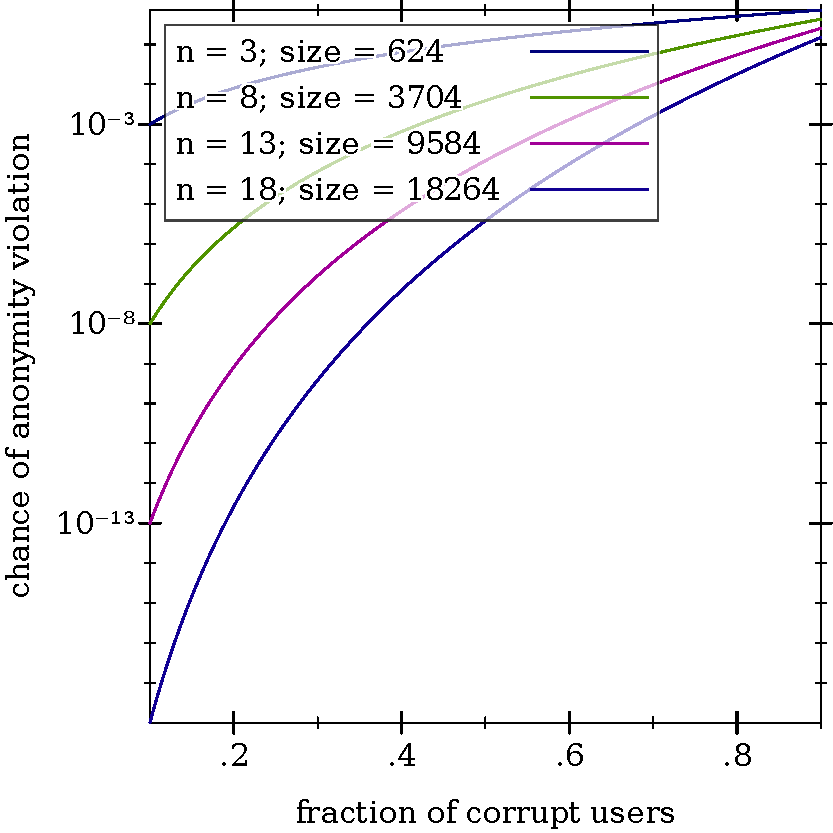
\includegraphics[width=0.66\linewidth]{bench/corruptfrac.pdf}
%     \caption{Privacy at different values for $n$ and BCH lock script sizes}
%     \label{fig:scriptsize}
% \end{figure}

% One possible concern with Astrape's performance behavior is that it establishes a tradeoff between privacy and performance. As $n$ increases, we get higher privacy but also higher per-hop overhead, especially for Bitcoin Cash-like blockchains with no support for recursive lock scripts. Let's quantify this effect to see whether or not overhead poses a serious barrier to high levels of privacy.

% To do so, we calculate the relationship between the fraction of corrupt users and the probability that at least intermediary in $n$ hops would be honest, for varying values of $n$. This is plotted in Figure \ref{fig:scriptsize}. We see that by increasing $n$ to about 10 we can reduce the chance of compromise to less than 1\% even if most of the nodes are corrupt, while still having script sizes around a dozen KB. Although such a script will be hundreds of times the size of an HTLC script, it is still small enough that communicating it across payment channels will not be a large burden.

% These script sizes do, however, cause large transaction costs in case transactions must settle on the blockchain. Thus, Astrape is probably not very suitable for on-chain coin-mixing services for blockchains with no recursive lock scripts. Other anonymous multi-hop transaction constructions, like the Fulgor or AMHL, may be more suitable in those situations.

\subsection{Statistical simulation}

Finally, we simulate the performance of Astrape on the network graph of Lightning Network.

\paragraph*{Setup}

\textbf{TODO: update info}

We set up a mainnet Lightning Network node using the \textsf{lnd} \cite{github2019lnd} reference implementation. We then used the \textsf{lncli describegraph} command to capture the network topology of Lightning Network in August 2019. This gives us a graph of 4767 nodes and 32219 edges. Finally, we randomly sample 1,000 pairs of nodes in the network and calculate the shortest paths between them. This gives us a randomly sampled set of real-life payment paths.
\begin{figure*}[t]
    \centering
    \begin{subfigure}[b]{0.3\textwidth}
        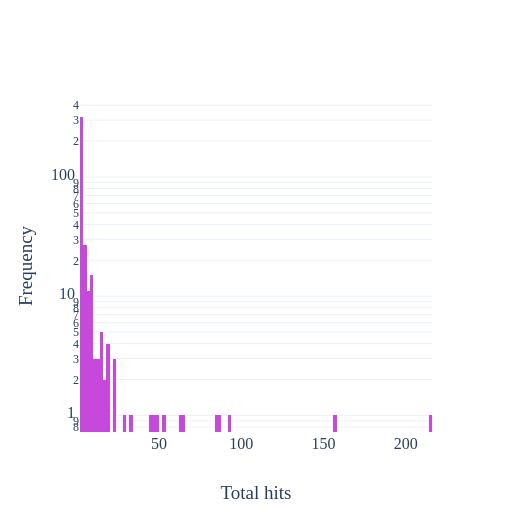
\includegraphics[width=\textwidth]{graphics/pl-hitcount.png}
        \caption{Hit distribution}
        \label{fig:hitcount}
    \end{subfigure}
    \begin{subfigure}[b]{0.3\textwidth}
        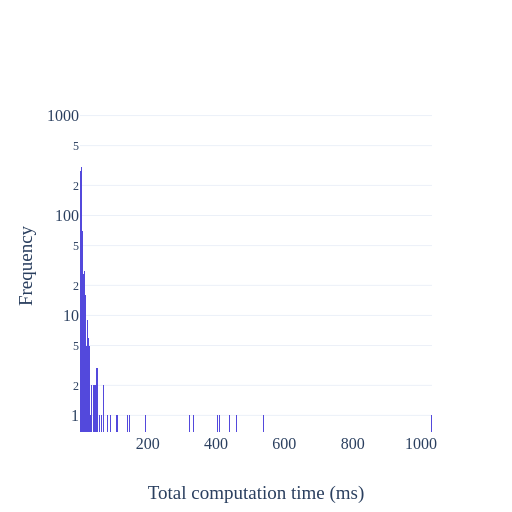
\includegraphics[width=\textwidth]{graphics/pl-cpuover.png}
        \caption{Total computation}
        \label{fig:cpuover}
    \end{subfigure}
    \begin{subfigure}[b]{0.3\textwidth}
        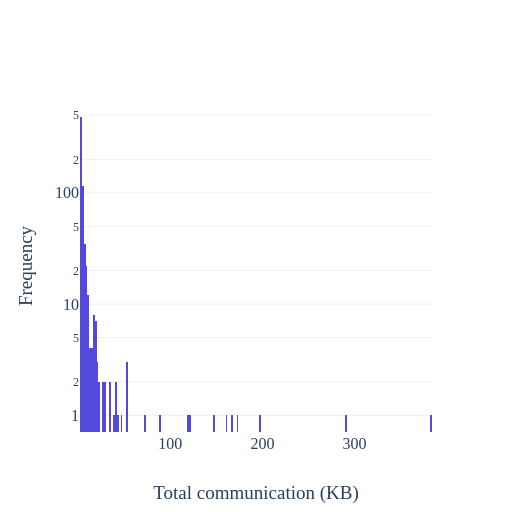
\includegraphics[width=\textwidth]{graphics/pl-commover.png}
        \caption{Total communication}
        \label{fig:commover}
    \end{subfigure}
    \caption{Overhead distribution}
\end{figure*}
\paragraph*{Path statistics}

\begin{figure}[H]
    \centering
    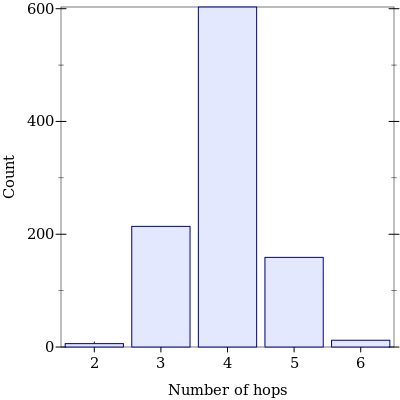
\includegraphics[width=0.66\linewidth]{graphics/hops.png}
    \caption{Distribution of shortest path lengths}
    \label{fig:hops}
\end{figure}

As we have previously shown, paths more than 10 hops long still have fairly small overhead even with non-recursive lock scripts, but much longer paths will cause unacceptably large unlock sizes. Will graph topology ever force payment to grow too long? Figure \ref{fig:hops} illustrates the distribution of lengths for our 1,000 randomly selected payment paths. On average, a payment path was 3.92 hops long, while even the longest payment paths were only 6 hops long. This indicates that shortest payment paths long enough to pose seriously ballooning worst-case overhead are practically nonexistent. A privacy-optimizing routing algorithm thus has ample room to deviate from shortest-path routing.

\paragraph*{Total scalability}

One important attribute we wish to explore with the LN topology is the total scalability of the network --- how fast can a PCN process transactions as a whole.

To do so, we keep track of how many times each node appears, or is ``hit'', in our 1,000 randomly selected payment routes. We see that the average number of hits is 1.97, but the vast majority of nodes are hit only once, while a few nodes are hit hundreds of times. This reflects that some nodes are unusually well-connected and act as ``hubs'' for a large fraction of all transactions. The distribution of hits is plotted in Figure \ref{fig:hitcount} as a log-linear histogram.

We then look at the \emph{distribution of overhead} in the network for both computation and communication. This is by calculating the total computation and communication cost for each node ``hit'' by the 1,000 random payments, using values from the Bitcoin Cash implementation. This allows us to calculate the resources required for the largest ``hubs'' in the network whose throughput limits that of the entire system.

Computation cost is plotted in Figure \ref{fig:cpuover}. We see that the most heavily loaded node in the entire network did around 1,000 ms of computation to process 1,000 transactions. This indicates that a PCN with the current Lightning Network topology will be able to process around 1,000 transactions a second with the largest hubs using commodity hardware. Such a throughput is orders of magnitude higher than that of typical blockchains and is within reach of many traditional payment systems. We note that the Lightning Network is still experimental; with a larger network this throughput will increase dramatically.

Communication cost is plotted in Figure \ref{fig:commover}. We used the quadratically increasing lock sizes of the unoptimized Bitcoin Cash implementation of Astrape, and assumed that all payments are settled through a worst-case ``collapse''. Even so, the total network load averages to only about 3.92 KB per node. The largest hubs' total load still do not exceed 400 KB. This illustrates that even though communication cost is worst-case quadratic in the number of payment hops, the bottleneck is actually computation, not communication --- with LN's topology major hubs will have saturated their processing power at 1,000 transactions per second, but would only have to transmit a meager 400 KB/s of data.

In summary, we see that Astrape's rather ``scary'' worst-case asymptotic performance poses no barriers to the total throughput of an Astrape-powered payment channel network. PCNs can enjoy the superb scalability associated with them just as easily with Astrape-powered privacy and security.

% \section{Future work} \label{sec:futurework}

% \subsection{Constant-space lock sizes}

% One interesting problem is whether or not an anonymous multi-hop transaction protocol using only ``conventional'' cryptography can work with constant lock size. Avoiding worst-case $O(n)$ lock sizes can allow the use of anonymous PCNs in applications where these lock sizes are problematic, such as on-chain coin laundering or bandwidth-constrained environments. But It seems unlikely that constant space usage is possible with Astrape-type constructions based on multi-hop HLTC and fraud proofs. There does not seem to be a straightforward way of securely committing to rightward $(r_i,s_i)$ parameters with sublinear witnesses.

% We wish to investigate as future work whether or not more sophisticated cryptographic commitment mechanisms, such as Merkle trees, can be used to eliminate the linearly growing fraud proofs.

% \subsection{Integrated private payment system}

% We are working on Astramel, a private payment system that combines Astrape-based PCNs with state-of-the-art anonymous communication protocols, on the Themelio \cite{themelio} cryptocurrency blockchain. A ``vertically integrated'' PCN designed from the ground up for strong anonymity has yet to be developed, and we believe that such a system will greatly enhance the usability of blockchain cryptocurrencies. Astramel will demonstrate that robust privacy is compatible with an easy user experience similar to that of traditional payment apps.

% \subsection{More robust notions of privacy}

% Privacy properties not captured by relationship anonymity, such as immunity from timing and other side-channel attacks, are notoriously hard to model. It's difficult to formalize a notion of security that captures time, long-term statistical correlations, etc.

% Unfortunately, anonymity breaks in anonymous communication systems have largely been attacks on these side channels. For instance, the Silk Road 2.0 darknet market was deanonymized largely from timing attacks \cite{silk}. In fact, for payment channel networks these side channels probably matter even more. First, payment volume is a small fraction of anonymous communication volume, making ``innocent'' transactions that an adversary can confuse targeted ones for rare. Moreover, payment metadata tends to be more sensitive on average than communication metadata, as they're sought after by motivated and powerful adversaries such as tax authorities.

% We urgently need a notion of payment channel privacy that captures the ``messy'' concepts of time information and distinguishability from other payments across the whole network --- not just distinguishability between two payments of the same length, time, etc intersecting at the same honest intermediary. More research into this area could lead to a much more robustly anonymous payment channel network that can truly replace less scalable alternatives such as physical cash and zero-knowledge-proof based cryptocurrencies like ZCash.

\section{Conclusion} \label{sec:conclusion}

Payment channel networks and other trust-minimizing intermediarized cryptocurrency payment systems currently deployed lack strong privacy and security guarantees. Existing research, although solving the privacy and security problems, introduce either stringent requirements on underlying blockchain semantics or nonstandard, difficult-to-port cryptographic primitives.

We presented Astrape, a novel PCN construction that breaks this conundrum. Astrape is the first PCN that achieves relationship anonymity and balance security with only black-box access to generic conventional cryptography. It relies on a general idea of using non-anonymous post-hoc fraud proofs to achieve balance security, while avoiding any information leaks when senders are not corrupt. This allows Astrape to avoid the zero-knowledge proofs used to achieve balance security in almost all other private PCNs, while having easily provable security poroperties.

Furthermore, we demonstrate that Astrape is practical to deploy in the real world. Performance is superior on average to existing private PCNs, even on blockchains that are unsuitable for free-form smart contracts. We also showed that Astrape achieves high scalability on a real-world payment channel network graph.

\bibliography{astrape}{}
\bibliographystyle{abbrv}

%\appendix 

% \section{Previous reviews from IEEE S\&P 2020}

% An earlier version of this paper has been submitted to and rejected from the IEEE Symposium on Security and Privacy, 2020. The main revisions made since then are as follows:
% \begin{itemize}
%     \item We created a formal mathematical model, GMHL, to describe Astrape.
%     \item Security models and proofs are under a formal adversary model and universal composability framework.
%     \item Notation was completely overhauled to be easier to read and more in line with existing work.
%     \item The main innovation of Astrape --- that it reduces cryptographic assumptions and is much easier to understand and implement than existing systems --- is highlighted.
%     \item Extensive copy-editing to improve language.
% \end{itemize}

% \subsection{Review 1: weak reject}

% \paragraph*{Paper summary}
% Astrape is a privacy improvement to the Hash Time Locked Contract (HTLC) paradigm used in modern Payment Channel Networks (PCNs). Rather than use a single hash preimage to ensure the atomicity of a payment across multiple off-chain transactions which can reveal the payment path, Astrape achieves off-chain atomicity with a different random value per off-chain transaction thus obfuscating the full payment path.

% \paragraph*{Strengths}
% This protocol derives its security from the security of a hash function. This makes it very simple construction to reason about and would be easier to implement than alternatives that rely on ZKPs or more complex protocols.

% The authors implemented a prototype of their protocol for Bitcoin-cash. Using this implementation they provide performance numbers for their protocol. This performance analysis shows that from a computation time perspective Astrape out performs AMHL (Anonymous Multi Hop Locks).

% A measure of the number of hops (i.e. path length) in the lightning network is provided. These measurements are useful for understanding what some of the parameters of their protocol would look like if deployed.

% \paragraph*{Weaknesses}

% Astrape does not currently compare well with AMHL (ECDSA) the main work in this space. AMHL (ECDSA) has constant sized lock and unlock sizes compared to Astrape unlock size that grows linearly in the number of hops and the BCH implementation of Astrape which has a lock size that is quadratic in the number of hops. The paper argues that the number of hops, n, is likely to be small, but even if n=3 that is still a worst-case of 624 Bytes unlocking size. In future work the paper discusses constant space lock sizes this feels like a critical feature to have.

% Astrape is only usable on blockchains that support a concatenate functionality i.e. OP\_CAT. On page 8 the paper states:

% "Astrape  requires  an  “append-like”  operation || that can take in two byte strings and combine them in a collision-resistant manner. This functionality is present in most Turing-incomplete scripting languages, including that of Litecoin and Bitcoin Cash. Unfortunately, the most popular cryptocurrency Bitcoin has disabled all of its string-manipulation opcodes"

% This appears to be incorrect. The Bitcoin script op code OP\_CAT which enables appending was disabled very early in Bitcoin's history (Aug 2010). It is BCH (Bitcoin-cash) not BTC (Bitcoin) which is the exception here in having OP\_CAT enabled and BCH only recently enabled OP\_CAT (in 2018).

% This means that this work as it is currently described is only applicable to BCH and BCH derived coins i.e. BCH and BSV. AMHL on the other hand is available on any cryptocurrency that supports nLocktime and ECDSA or Schnorr signatures.

% Related work section is missing a comparison with recent work A2L

% \subsection{Review 2: weak reject}

% \paragraph*{Paper summary} The paper proposes a protocol for anonymous payment channel networks (PCN) that relies only on signatures and hash functions, and is claimed to achieve better security and privacy guarantees than currently deployed solutions.

% \paragraph*{Strengths} relies on simple building blocks only, efficient implementation

% \paragraph*{Weaknesses} absence of formal or sufficiently detailed security and functional properties make it hard to understand and verify the properties; informal protocol description only

% \subsection{Review 3: weak accept}

% \paragraph*{Paper summary} This paper describes Astrape, a design for a payment channel network that preserves relationship anonymity: an adversary cannot distinguish between two same-sized payments with the same path length as long as they intersect at one honest user.  It does so using simple cryptographic primitives and fraud proofs.

% \paragraph*{Strengths} This design is very clever, and it is well-evaluated.  The evaluation shows good performance despite the size of the locks scaling quadratically with the length of the path.

% \paragraph*{Weaknesses} It's unfortunate this doesn't work with Bitcoin as it limits applicability. It's hard to compare to [7] and [8] because they are compatible with Bitcoin.

% One concern I have is how to determine fees correctly. In the worst, case, where the sender is malicious, one must pay for a much larger transaction chain than if the sender is honest.  This makes fee estimation hard.

% I found the paper difficult to understand.
\end{document}